\section{Introduction}
\begin{frame}{}
    \LARGE Video Learning \& Generation: \textbf{Introduction}
\end{frame}

\begin{frame}[allowframebreaks]{What is Video Data?}
    \begin{itemize}
        \item \textbf{Video} is a sequence of images (frames) captured over time.
        \item Each frame is a static image, but the sequence captures motion and temporal dynamics.
        \item Videos can be continuous (e.g., surveillance footage) or discrete (e.g., video clips).
        \item Key components:
        \begin{itemize}
            \item Frame rate: number of frames per second (FPS).
            \item Resolution: dimensions of each frame.
            \item Duration: total length of the video.
        \end{itemize}
    \end{itemize}
\framebreak
    \begin{figure}
        \centering
        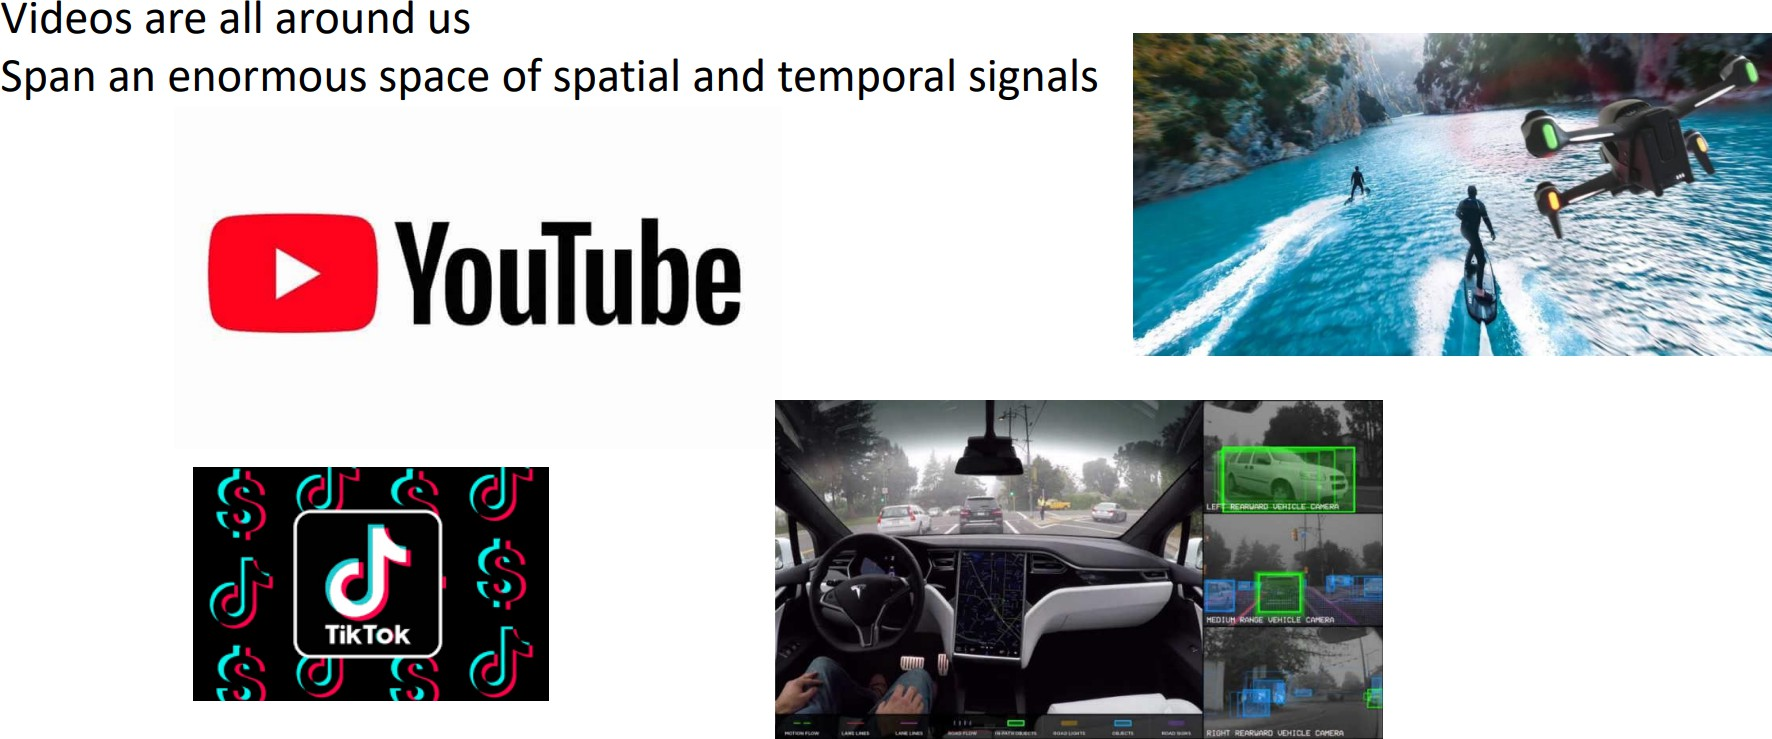
\includegraphics[width=1\textwidth,height=0.9\textheight,keepaspectratio]{images/video/slide_2_1_img.jpg}
    \end{figure}
\framebreak
    \begin{figure}
        \centering
        \fetchconvertimage{https://onlinehelpstaticcontents.avs4you.com/en/images/videoeditor/videoproperties.png}{images/video/video_properties.png}{width=1\textwidth,height=0.9\textheight,keepaspectratio}
    \end{figure}
\framebreak
    \begin{figure}
        \centering
        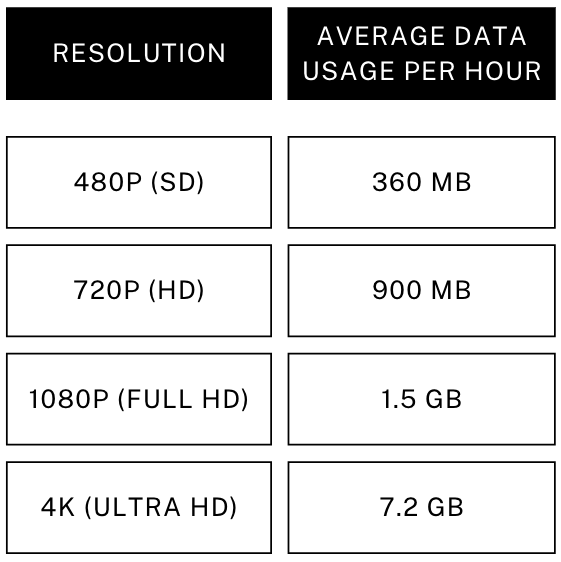
\includegraphics[width=1\textwidth,height=0.9\textheight,keepaspectratio]{images/video/video_properties-2.png}
    \end{figure}
\framebreak
    \begin{figure}
        \centering
        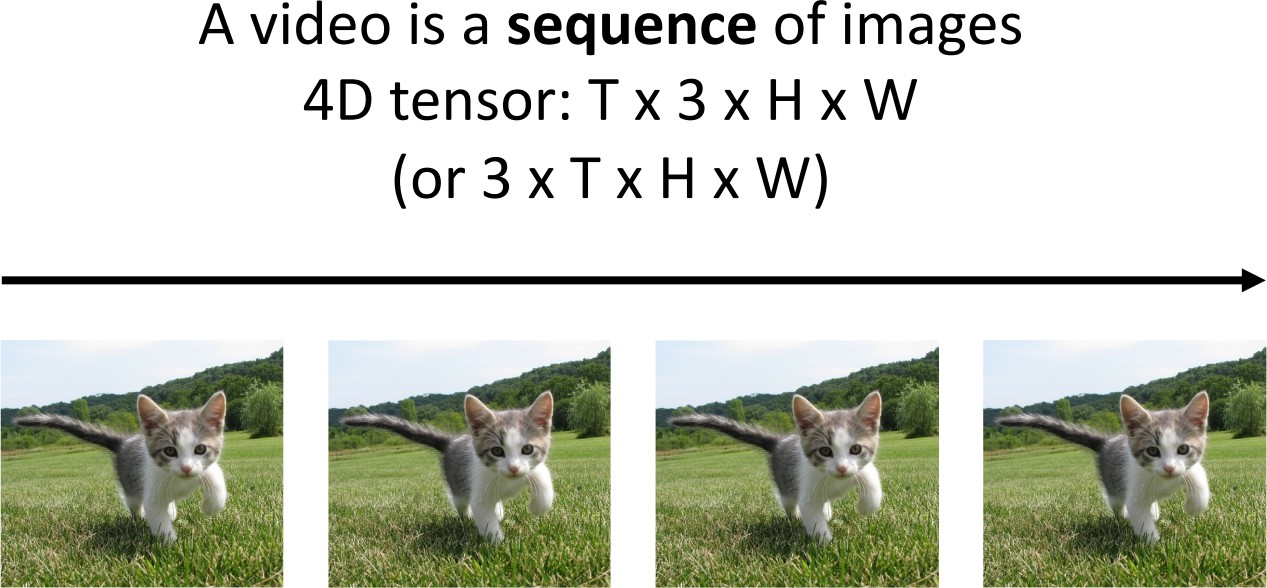
\includegraphics[width=1\textwidth,height=0.9\textheight,keepaspectratio]{images/video/slide_3_1_img.jpg}
    \end{figure}
\end{frame}

\begin{frame}[allowframebreaks]{Camera Properties}
    \begin{itemize}
        \item Cameras capture video data with various properties that affect quality and usability.
        \item Key properties include:
        \begin{itemize}
            \item \textbf{FPS (Frames per Second):} Determines the temporal resolution of the video; higher FPS captures smoother motion.
            \item \textbf{Spatial Resolution:} Refers to the pixel dimensions of each frame (e.g., 1920x1080); affects image detail.
            \item \textbf{Field of View (FOV):} The angular extent of the observable scene captured by the camera; wide FOV covers more area.
            \item \textbf{Depth Sensors:} Devices like RGB-D cameras and LiDAR provide depth information, enabling 3D scene understanding.
        \end{itemize}
    \end{itemize}
\framebreak
    \begin{figure}
        \centering
        \fetchconvertimage{https://home-cdn.reolink.us/wp-content/uploads/2023/06/200657281687244248.0603.jpg}{images/video/camera-fps.png}{width=1\textwidth,height=0.9\textheight,keepaspectratio}
    \end{figure}
\framebreak
    \begin{figure}
        \centering
        \fetchconvertimage{https://kintronics.com/wp-content/uploads/2022/08/FOV.jpg}{images/video/camera-fov.png}{width=1\textwidth,height=0.9\textheight,keepaspectratio}
    \end{figure}
\framebreak
    \begin{figure}
        \centering
        \fetchconvertimage{https://home-cdn.reolink.us/wp-content/uploads/2019/08/analog-vs-ip-security-camera-resolution.jpg}{images/video/camera-res.png}{width=1\textwidth,height=0.9\textheight,keepaspectratio}
    \end{figure}
\framebreak
    \begin{figure}
        \centering
        \fetchconvertimage{https://www.researchgate.net/publication/308705183/figure/fig1/AS:411466659319808@1475112704288/top-The-hardware-scheme-of-the-RGB-D-sensor-sensor-with-RGB-camera-and-Depth-camera.png}{images/video/camera-rgbd.png}{width=1\textwidth,height=0.9\textheight,keepaspectratio}
    \end{figure}
\end{frame}

\begin{frame}[allowframebreaks]{What Does Temporal Mean?}
    \begin{itemize}
        \item \textbf{Single Frame:} Static content; no motion cues.
        \item \textbf{Short Clip:} Captures motion trajectories.
        \item \textbf{Temporal Window:} Enables extraction of velocity and acceleration.
        \item \textbf{Temporal Features:} Techniques such as frame differencing and optical flow capture motion information.
    \end{itemize}
    \begin{figure}
        \centering
        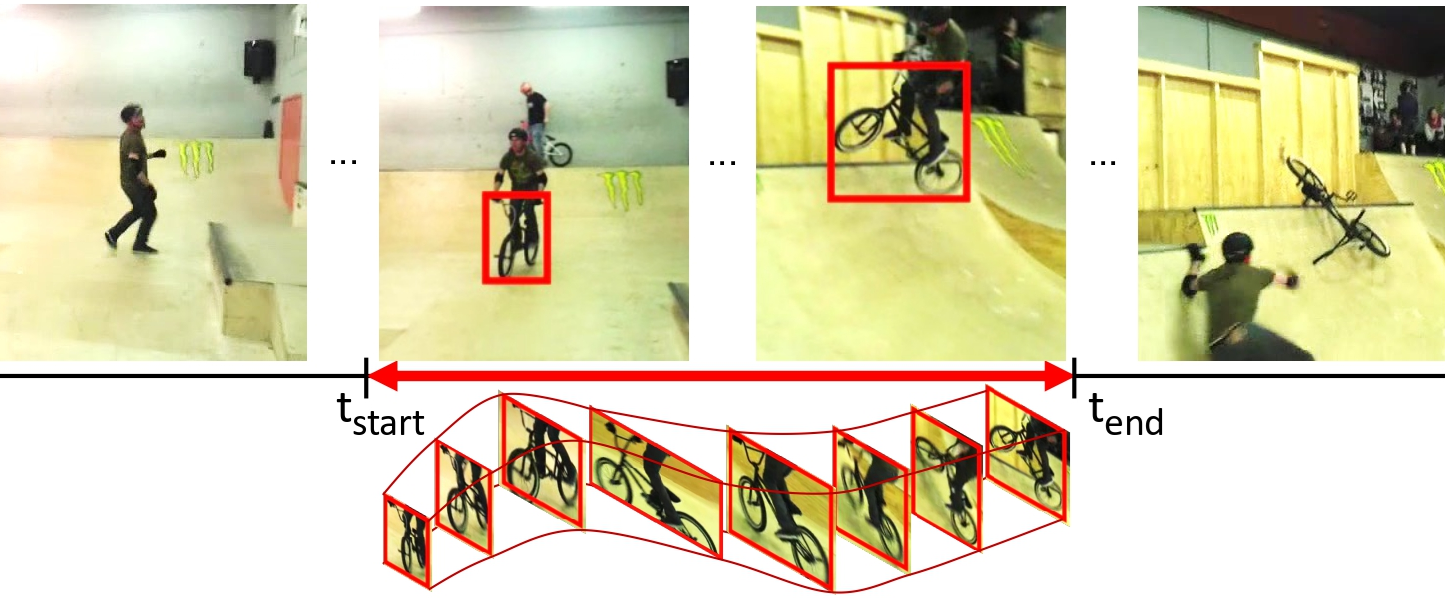
\includegraphics[width=1\textwidth,keepaspectratio]{images/video/temporal_features.png}
        \caption*{Illustration of temporal features in video: single frame, short clip, and motion extraction.}
    \end{figure}
\end{frame}